\chapter{Architecture}

\label{chap:Architecture}
This chapter presents the architectural design of the proposed model, \textbf{TakuNet}, developed to support fast and memory-efficient neural architecture search (NAS), particularly for embedded and resource-constrained environments. 
TakuNet is a lightweight convolutional neural network originally designed for efficient real-time inference on resource-constrained platforms \cite{TakuNet}.
The core design goal of TakuNet is to minimize the number of parameters and computational cost without significantly sacrificing accuracy.

This architecture has been used as a template because, according to recent studies, it requires significantly fewer parameters for a given dataset compared to other common architectures such as SqueezeNet and MobileNet \cite{TakuNet}. This makes it more feasible to develop a model that fits within our deployment environment.

This architecture is used throughout the NAS algorithm with the goal of identifying the optimal hyperparameters and optimizers for each layer. In this thesis, no additional layers are introduced; instead, only the existing parameters are shuffled. This decision was made due to time constraints, as introducing new layers would have significantly expanded the search space and increased the computational complexity of the NAS process.

We begin with an overview of the high-level components of TakuNet, followed by a detailed breakdown of its internal building blocks. Additionally, we discuss the model’s memory-aware design, training-time regularization strategies, and how it integrates with a NAS framework. Finally, we explain the deployment process and analyze key performance metrics, including floating point operations (FLOPs), memory footprint, and quantized model accuracy.


\section{Overview of TakuNet}

This work introduces an enhanced version of the architecture, specifically adapted for Neural Architecture Search (NAS) optimization. In the original TakuNet study, both the network architecture and the optimization function were determined through manual trial-and-error, which may not yield optimal results across different datasets. Rather than relying on a fixed architecture tailored to a specific dataset, our approach treats the model parameters as tunable hyperparameters. These are automatically evolved to maximize performance while adhering to the constraints of embedded systems.

The goal is to integrate architectural efficiency, automated design exploration via NAS, and hardware-aware optimization to develop a deep learning model that is both highly deployable and energy-efficient.

An illustration of our Architecture can be depicted in Figure~\ref{fig:TakuNet}

\section{Modular Building Blocks}


\subsection{Normalization Block}

\begin{sloppypar}
A core component used throughout the proposed architecture is the \textbf{Normalization Block}. It plays a critical role in preparing activations for both stable training and efficient deployment on low-precision hardware.
\end{sloppypar}

Specifically, this block standardizes the outputs of convolutional layers and ensures that the resulting activations are well-suited for quantization.


The Normalization Block consists of the following layers:

\begin{itemize}

    \item \textbf{Batch Normalization:} This layer is applied immediately after the convolutional operation. Its primary purpose is to normalize the intermediate activations by adjusting and scaling them such that they have zero mean and unit variance across the mini-batch. This normalization mitigates the issue of \textit{internal covariate shift}, where the distribution of inputs to each layer changes during training, thus destabilizing the learning process. By maintaining consistent activation distributions, Batch Normalization allows the network to use higher learning rates, accelerates convergence, and provides a mild regularization effect that can reduce the need for other forms of regularization such as dropout \cite{BatchNorm}.

    
    \item \textbf{ReLU6 Activation:} Following normalization, a ReLU6 non-linearity is applied. This is a variant of the standard ReLU function that caps the output at 6. By limiting the activation range to $[0, 6]$, ReLU6 enhances robustness to activation outliers and facilitates quantization-aware training. On devices with limited numerical precision (e.g., 8-bit microcontrollers), this bounded range leads to more accurate and efficient quantization \cite{ConvNetworksMobileNets}.
\end{itemize}

\subsection{Stem Block}

The Stem Block of the proposed architecture serves as the initial processing unit, tasked with transforming raw input images into a compact, information-rich feature representation while significantly reducing computational complexity. 

\begin{itemize}

    \item The block begins with a standard Conv2D layer that applies a set of learnable filters across the input, capturing fundamental visual patterns such as edges, textures, and color gradients. This layer employs a small kernel size and a stride, enabling early dimensional downsampling and increasing the channel depth (e.g., from 3 RGB channels to 40 feature maps), thereby balancing feature extraction richness with computational efficiency.
    
    \item The output of the full Conv2D layer is then passed through the previously discussed Normalization Block to ensure standardized activations suitable for subsequent processing and quantization.
    
\end{itemize}

The use of a standard convolutional layer followed by normalization ensures that the Stem Block effectively extracts low-level visual features while maintaining stable and quantization-friendly activations. It is essential to use a Full Convolution Layer with a stride > 1,  as the first layer of our Network, as processes all input channels together (e.g., RGB). In addition, starting with DWConv might lead to weak gradients or poor early feature learning, especially on small datasets like CIFAR-100.A single full Conv2D gives a denser representation, stabilizing the early stages of training 
\cite{ConvNetworksMobileNets}


\begin{comment}
To further improve the generalization capabilities of the model, an Adaptive Dropout layer is optionally applied. Unlike standard dropout, Adaptive Dropout dynamically adjusts the probability of drop during training, ensuring stronger regularization in the early training phases while allowing convergence toward optimal feature representations later and potentially assist avoid overfitting \cite{Dropout} .
\end{comment}




\subsection{Taku Block}

The \textbf{Taku Block} serves as the principal feature extraction module within the TakuNet architecture. It is specifically designed for efficient and progressive spatial feature refinement, while maintaining an extremely lightweight footprint—making it ideal for deployment in resource-constrained embedded systems.

Unlike conventional convolutional blocks that rely on computationally expensive standard convolutions (Conv2D), the Taku Block exclusively leverages \textbf{Depthwise Convolution (DWConv)} layers. These layers operate on each input channel independently, significantly reducing both the number of parameters and the number of floating-point operations (FLOPs) compared to full convolutions, while still preserving spatial feature learning capabilities.

The internal structure of the Taku Block consists of the following key components:

\begin{itemize}
    \item \textbf{Depthwise Convolution:} 
    Unlike standard convolution, which applies a single filter across all input channels simultaneously (mixing spatial and cross-channel information), Depthwise Convolution operates by applying a distinct spatial filter to each input channel independently. 
    
    Given an input tensor with $C$ channels, Depthwise Convolution uses $C$ separate filters—each of size $k \times k$—one per channel ( Total Parameters: $k \times k \times C$ ). This results in a significant reduction in the number of parameters and computational operations compared to traditional convolutions, which would require $k \times k \times C \times N$ parameters for $N$ output channels.
    
    The main purpose of Depthwise Convolution is to extract spatial features (e.g., edges, corners, textures) within each channel independently, without performing any cross-channel mixing. This spatial filtering is particularly useful in the early and intermediate stages of lightweight architectures, where reducing computational cost is critical for real-time or embedded deployment.

    \textbf{Tip for intuition:} Imagine the input image is a cat. Each input channel represents a different filtered version of that image — one might emphasize texture, another might capture color gradients, and another might highlight edges. Depthwise Convolution applies a unique spatial filter to each channel independently, like assigning a specialist to analyze specific parts of the cat: one filter might focus on detecting whiskers, another on ear contours, and another on the tail. None of these filters share information directly with the others, which keeps the computation light and efficient while still capturing meaningful spatial details.

     Overall, Depthwise Convolution enables spatial learning at low cost, making it ideal for embedded and real-time deep learning applications.


    \item \textbf{Normalization Block}

    \item \textbf{Skip Connection (Residual Addition):} Skip connections, also known as residual connections, are a key feature introduced in ResNet~\cite{zhou2021resnext}. In this design, the output of a series of operations (e.g., convolutions, activations) is added element wise to the original input of the block. This yields an output of the form:

\[
\text{Output} = F(x) + x
\]

where \( F(x) \) is the learned transformation and \( x \) is the original input.

This technique offers several critical advantages:

\begin{itemize}
  \item \textbf{Facilitates Gradient Flow:} During backpropagation, gradients can pass directly through the shortcut (\(+x\)) without getting diminished. This helps reduce the vanishing gradient problem in very deep networks.
  
  \item \textbf{Easier to Learn Identity Mappings:} If the optimal output is similar to the input, the network can simply learn \( F(x) \approx 0 \), effectively making the block skip itself. This is much easier than learning an identity mapping from scratch.
  
  \item \textbf{Preserves Input Information:} Important features in the input—such as edges or textures—can propagate to deeper layers without being lost, which can improve overall representational power.
  
  \item \textbf{Enables Deeper Architectures:} Without residual connections, training networks with dozens or even hundreds of layers is extremely difficult due to optimization challenges. Residual connections make this not only feasible but also stable.
\end{itemize}

\subsubsection*{Practical Analogy}
\textit{Think of it like writing a report where you keep a copy of your original draft and add comments or corrections (\( F(x) \)) on top of it. Instead of rewriting everything from scratch, you retain the core idea (\( x \)) and just refine it. If your edits (\( F(x) \)) are not useful, you can simply ignore them, preserving the original version.}
\end{itemize}

By integrating these components, the Taku Block balances efficiency and performance, making it a powerful building block for modern lightweight convolutional neural networks.

\begin{comment}
  Tip!!
Think it like that: If the image is a cat
Then each Block is trying to learn Spatial Features
Lets say the first is the whispers, the second is for the ears and so on
  
\end{comment}

\subsection{Downsampler Block}

The \texttt{DownSampler} block in \texttt{TakuNet} is designed for efficient feature transformation with minimal computational overhead, particularly important after the Depthwise Convolution layers used in preceding blocks. It employs a **grouped pointwise convolution**, dynamically adjusting the number of groups based on both the input/output channels and the network depth. Specifically, the number of groups is computed as the nearest valid integer to:

\[
\left\lfloor \frac{\texttt{Input\_Channel} + \texttt{Output\_Channel}}{\texttt{stages number}} \right\rfloor
\]

Here, \texttt{Input\_Channel} refers to the output of the previous \texttt{DownSampler} or the initial stem block, while \texttt{Output\_Channel} corresponds to the output of the last \texttt{TakuBlock}. This dynamic grouping ensures both divisibility and computational efficiency.

A kernel size of \(1 \times 1\) is used in the grouped convolution, making it a pointwise operation that linearly projects feature channels at each spatial location. This enables channel-wise feature interaction without spatial correlation, maintaining resolution while significantly reducing computation~\cite{PointwiseGroupedCon}. 
If the input channels cannot be evenly divided, the block falls back to a standard pointwise convolution (i.e., groups = 1), ensuring robustness.

The \texttt{DownSampler} block contains the following layers, in order:

\begin{itemize}
  \item \textbf{Grouped Pointwise Convolution} (\(1 \times 1\)): performs efficient channel-wise transformations.
  \TODO{Maybe add the above information to the Grouped Poinwise Convolution}
  \item \textbf{Normalization Block}
  
  \item \textbf{Pooling Layer}:
  \begin{itemize}

    \item \textbf{Max Pooling} is applied during the earlier stages of the network to perform aggressive spatial downsampling. It selects the maximum value from small local regions (typically $2 \times 2$ patches), effectively halving both the height and width of the feature map when using a stride of 2. This results in a $75\%$ reduction in the number of spatial elements (e.g., $32 \times 32 \rightarrow 16 \times 16$), which in turn reduces the computational load for subsequent layers by up to \textbf{4×} per stage. Beyond reducing memory and FLOPs, it also preserves only the most salient features—like edges or corners—helping the network learn robust low-level representations with minimal overhead.

    \item \textbf{Average Pooling} is used in the final stage to produce a smoother, generalized spatial representation of the feature map. Conceptually, Average Pooling slides a small window (e.g., $2 \times 2$) across the spatial dimensions of the input feature map and replaces each window with the \emph{average} of its values. Unlike Max Pooling, which retains only the strongest activation in each region, Average Pooling captures the overall trend or intensity level across that region.

    This operation serves as a form of spatial smoothing: it diminishes the influence of outliers and noisy activations while retaining a more balanced view of the learned features. As a result, the model develops a more holistic understanding of the input, which is particularly beneficial in the final stages where high-level semantic features (like “cat-ness” or “airplane-ness”) are dominant.
    
    Like Max Pooling, Average Pooling also reduces the spatial dimensions. For example, applying a $2 \times 2$ window with a stride of 2 on an $8 \times 8$ feature map will reduce it to $4 \times 4$, effectively cutting the spatial resolution by $75\%$. This reduction significantly decreases the number of computations and memory usage for subsequent layers (e.g., dense classifiers), while still preserving meaningful abstracted information. This not only reduces the risk of overfitting, but also improves inference efficiency on resource-constrained devices.
  \end{itemize}
  
    \item \textbf{Layer Normalization}: applied at the end of the \texttt{DownSampler} block to improve the robustness and stability of activations. Unlike Batch Normalization, which computes statistics across a batch of samples, Layer Normalization normalizes the activations within each individual sample by computing the mean and variance across its feature dimensions. This makes it highly effective in real-time or embedded environments, where batch sizes are small or even equal to one. By keeping the activations well-scaled and centered, Layer Normalization ensures that the following layers receive inputs in a stable range, reducing sensitivity to input shifts and enhancing generalization, especially under deployment constraints.
    
\end{itemize}

\subsection{Refiner Block}

The \texttt{Refiner} block serves as the final stage of the \texttt{TakuNet} architecture. It takes as input the output tensor of the final \texttt{DownSampler} block, which typically has a significantly reduced spatial dimension but enriched channel-wise features. The goal of the \texttt{Refiner} is to perform final feature distillation and produce class probabilities through a softmax layer.

The block is composed of the following steps:

\begin{itemize}
    \item \textbf{Depthwise Convolution}: A spatial depthwise convolution is applied to refine local feature responses while maintaining channel-wise separation. This operation enables low-cost spatial filtering tailored to each feature channel independently.
    
    \item \textbf{Batch Normalization}: This layer stabilizes training and accelerates convergence by normalizing the feature distributions after convolution. It ensures that the scale of the activations remains consistent.
    
    \item \textbf{Adaptive Dropout (Post-Convolution)}: A custom \texttt{AdaptiveDropout} layer is applied to mitigate overfitting and introduce regularization right after the depthwise convolution. The dropout rate is dynamically adjusted based on training behavior, making the model more robust during final refinement.
    
    \item \textbf{Global Average Pooling (GAP)}: This operation collapses the spatial dimensions by computing the average activation for each channel. The result is a compact feature vector that summarizes global information across the entire spatial domain.
    
    \item \textbf{Adaptive Dropout (Post-GAP)}: A second \texttt{AdaptiveDropout} layer is applied to the pooled vector. As this vector will be directly passed to the final classification layer, regularizing it helps to prevent overfitting on high-level semantic representations.
    
    \item \textbf{Dense Layer with Softmax Activation}: The final layer is a fully connected \texttt{Dense} layer with as many units as the number of output classes. A softmax activation is applied to produce normalized class probabilities, which form the model's prediction.
    
\end{itemize}

This block acts as the final decision-making stage of the network. By combining spatially aware filtering, global summarization, and regularization, the \texttt{Refiner} ensures that the most relevant features are passed to the classifier. Its lightweight design and careful placement of dropout layers make it especially suitable for resource-constrained environments where both accuracy and efficiency are critical.



\begin{figure}[ht]
    \centering
    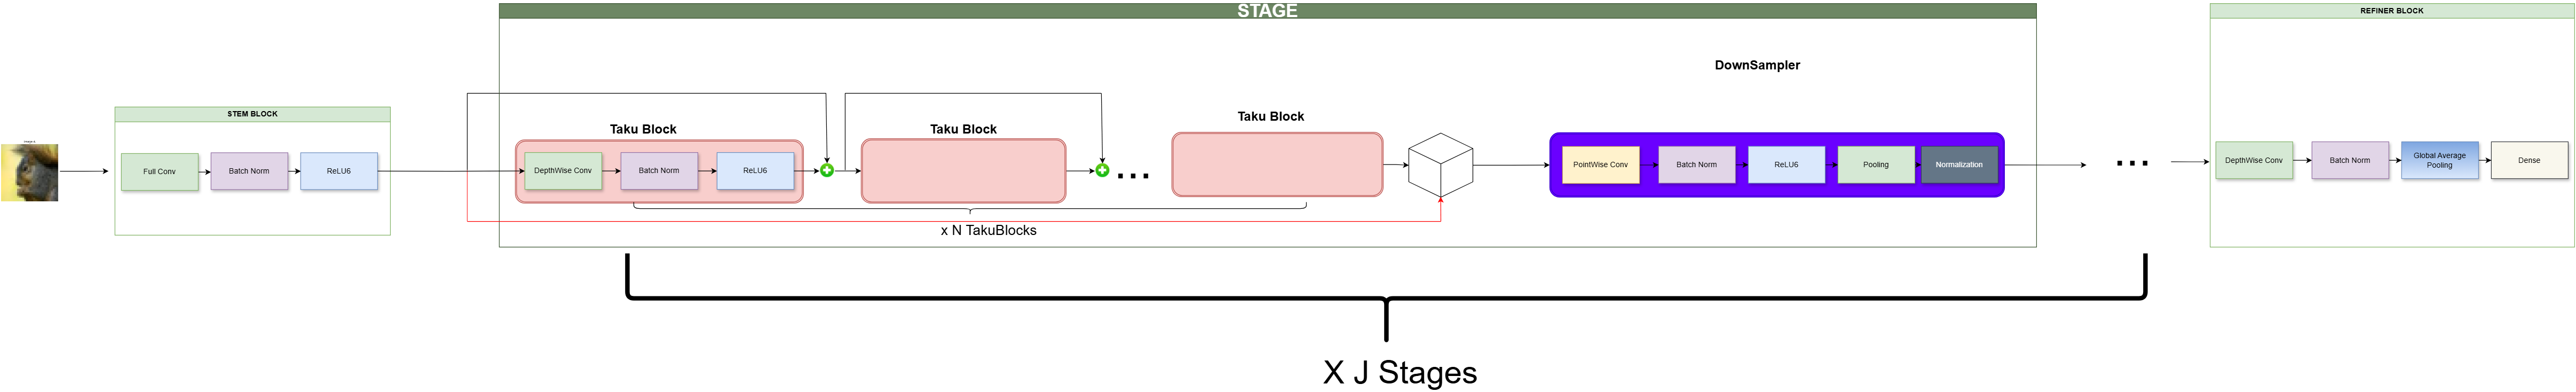
\includegraphics[width=\linewidth]{Pictures/TakuNet.png}
    \caption{Enhanced TakuNet}
    \label{fig:TakuNet}
\end{figure}


\section{Enchantments in TakuNet model}

\subsection{Adaptive Dropout}

A key contribution of this work is the integration of an \textit{Adaptive Dropout} mechanism, designed to dynamically adjust the dropout rate during training. Traditional dropout applies a fixed probability of deactivating neurons to prevent overfitting. However, selecting an optimal dropout rate a priori can be challenging, especially in resource-constrained environments where overfitting behavior may vary across training stages and datasets.

The Adaptive Dropout mechanism in TakuNet addresses this limitation by treating dropout as a dynamic process. Each Adaptive Dropout layer begins with a low dropout rate and increases it only when overfitting is detected—specifically, when the training accuracy significantly exceeds the validation accuracy over a sustained period. This behavior is implemented using a custom callback that monitors training metrics and incrementally raises the dropout rate for selected layers, subject to layer-specific limits.

\paragraph{Placement of Dropout Layers.} Dropout is strategically applied in the following parts of the architecture:
\begin{itemize}
    \item \textbf{Stem Block:} This initial layer extracts low-level features from the input. Applying a mild dropout here ensures that early representations do not become overly specialized, improving generalization from the outset.
    
    \item \textbf{Taku Blocks (Main Stages):} These depthwise convolutional blocks form the core of the architecture and are repeated multiple times. Dropout in these layers is more heavily used because they contain most of the model’s representational capacity and are more prone to memorization. Since they are deeper in the network, they tend to accumulate overfitting more readily, making them ideal candidates for adaptive regularization.
    
    \item \textbf{Refiner Block:} This final stage performs global feature aggregation and classification. Due to its dense connectivity and proximity to the output layer, it is particularly sensitive to overfitting. Therefore, dropout here typically starts with a higher rate and may increase more aggressively if overfitting is detected.
\end{itemize}

\paragraph{Layer-Specific Behavior.} Not all layers benefit equally from dropout. For instance, early convolutional layers (like those in the stem block) are less likely to overfit, so they receive smaller dropout increments and have lower maximum limits. Conversely, later layers—especially those with dense or global receptive fields—are more prone to overfitting and thus are configured with higher initial dropout rates and greater allowed increases. This design mimics the intuition that deeper layers encode more abstract (and potentially dataset-specific) features, and hence require stronger regularization.

\paragraph{Deployment Considerations.} Once training is complete, all Adaptive Dropout layers are "frozen" into standard Dropout layers with fixed rates. This makes the architecture compatible with deterministic inference pipelines, such as TFLite conversion and deployment to low-power embedded systems.

\paragraph{Benefits.} The Adaptive Dropout mechanism improves generalization without extensive manual tuning and makes the model more robust across datasets. It also ensures that the resulting model remains compact, efficient, and deployable on resource-constrained hardware platforms.

